\documentclass[a4paper,titlepage]{article}
\usepackage[]{mcode}
\usepackage{natbib}
\usepackage{graphicx}
\usepackage{hyperref}
\usepackage{amsthm}
\usepackage{amsmath}
\usepackage[margin=2cm]{geometry}

\begin{document}

\begin{titlepage}
	\newcommand{\HRule}{\rule{\linewidth}{0.5mm}}
	\center

	%------------------------------------------------
	%   Logo
	%------------------------------------------------

	
\includegraphics[width=0.2\textwidth]{Crest.jpg}\\[1cm]

	%------------------------------------------------
	%	Headings
	%------------------------------------------------

	\textsc{\LARGE University of Exeter}\\[1.5cm]

	\textsc{\Large College of Engineering, Mathematics and Physical Sciences}\\[0.5cm]

	\textsc{\large ECM3735 - Group 8}\\[0.5cm]

	%------------------------------------------------
	%	Title
	%------------------------------------------------

	\HRule\\[0.4cm]

	{\huge\bfseries Finding the optimal strategy for the dice game `Pig'}\\[0.4cm]

	\HRule\\[1.5cm]

	%------------------------------------------------
	%	Authors
	%------------------------------------------------

	\LARGE\textit{Authors}\\
	\begin{minipage}{0.4\textwidth}
		\begin{flushleft}
			\large
			S. \textsc{Bayliss}\\
			A. \textsc{Dunford}\\
			E. \textsc{Morison}\\
			J. \textsc{Peet}\\
			L. \textsc{Sutton}
		\end{flushleft}
	\end{minipage}
	~
	\begin{minipage}{0.4\textwidth}
		\begin{flushright}
			\large
			C. \textsc{Crawford}\\
			R. \textsc{Jones}\\
			C. \textsc{Nash}\\
			A. \textsc{Smith}
			\vspace*{10pt§}
		\end{flushright}
	\end{minipage}

	\vfill\vfill
	\textit{Supervisor}\\
	Dr. B. \textsc{Cooper}

	%------------------------------------------------
	%	Date
	%------------------------------------------------

	\vfill\vfill\vfill

	{\large\today}
	\vfill

	%------------------------------------------------
	%	Abstract
	%------------------------------------------------

	\newpage
	\begin{abstract}
	\textit{Insert abstract here}
	\end{abstract}
\end{titlepage}

	%------------------------------------------------
	%	Contents
	%------------------------------------------------

\tableofcontents
\newpage

\section{Introduction}

\subsection{Aims and Objectives}
josh

\subsection{Basics of Pig}
`Pig' is a turn based dice game played by 2 people rolling a die. The number on the die signifies the points gained on that roll,
which are collated in a sum total of points for the turn. These points can be banked to bring a players turn to an end.
However, the points in this rolling total can be lost if the player rolls a $1$, this will also automatically bring their turn to an end.
The aim of the game is to be the first player to have a banked total of points greater than or equal to $100$.
\\
\\
Many different strategies can be used in Pig. For example, a simple strategy would be to roll until passing a turn score of 20, then banking.
A strategy can be thought of as the choice to either roll the dice, or bank the turn score, at any game state.

A game state is defined by the current position of the game, my banked score, your banked score, and my turn score.
These three scores vary between zero and 100. The mistake would be to assume that this means there are $100\times100\times100 = 1$ Million
game states. The reason this is not true is because many are not possible. Take a banked score of $90$ and a turn score of $50$ for example,
this game would have ended a long time ago when the player reached a turn score of $10$ winning them the game! This could be called an impossible
game state, because it is not possible to reach this state, playing by the rules of the game. Another type of impossible game state is
with a turn score of $1$. The smallest turnscore larger than $0$ that a player can have is by rolling a $2$, giving them a turn score of $2$.

Let us now define a strategy as an array of choices, 1s for rolling, and 0s for banking, where the array is 3 dimensional, and containing every
possible game state.
Does this let us define every possible strategy or are there more variables to consider?
If this does define every strategy, the next big question, and the main focus of this paper, is what is the best strategy to play?
What strategy is most likely to win against any other, and be crowned the Optimal Strategy for the dice game pig.
\\
\\
At any gamestate it is possible to produce linear equations to determine if it is better to roll or bank by looking at the probability of winning from that gamestate.
Suppose I have 2 strategies A and B. Consider that it is A's turn and we are in position ($i,j,k$) where $i$ is A's banked points,
$j$ is B's banked points, and $k$ is A's sum total of points so far on this turn. Let $P_{ijk}$ denote the probability of A winning
from the current position and $Q_{jik}$ denote probability of B winning from the equivalent position (Note that the position of $j$ and $i$ have swapped because it is
from the perspective of each player). Then, \begin{equation}\label{1.2.1.a}
p_{ijk} = \dfrac{1}{6} (1-Q_{ij0}) + \dfrac{1}{6}\sum^{6}_{r=2}P_{ijk+r}
\end{equation}
 if A rolls and
 \begin{equation}\label{1.2.1.b}
 p_{ijk} = 1-Q_{jik}
 \end{equation}
 if A banks their points.
 \\
 \\
 These equations and this way of thinking about gamestates and strategies is key to our exploration further for an optimal strategy.

\subsection{Nellers Work}
In \textit{Dice Games Properly Explained}, Reiner Knizia takes the view of each roll of the die in `pig' as a bet of not rolling a $1$.
He viewed the best strategy as ``Whenever your accumulated points are less than 20, you should continue throwing, because the odds are in your favour.''\cite{knizia2010dice}.
However, Todd W Neller stated ``\textit{risking points is not the same as risking the probability of winning.}''\cite{neller2004optimal},
from this Neller proceeded to find a more optimal solution for `pig' by taking the maximum of equation \ref{1.2.1.a} and equation \ref{1.2.1.b}.
This was not possible however as he ended up with an equation of the form $x=$max$ (A_1 x+b_1,A_2 x+b_2)$ for which there is no known general method.
As a result Neller implemented value iteration to calculate an accurate estimate for the probabilities at each position $(i,j,k)$ for both bank and roll.
Figure \ref{figure1} shows the resulting optimal strategy where you should roll if you are below the surface of the graph and bank if above.

\begin{figure}
\centering
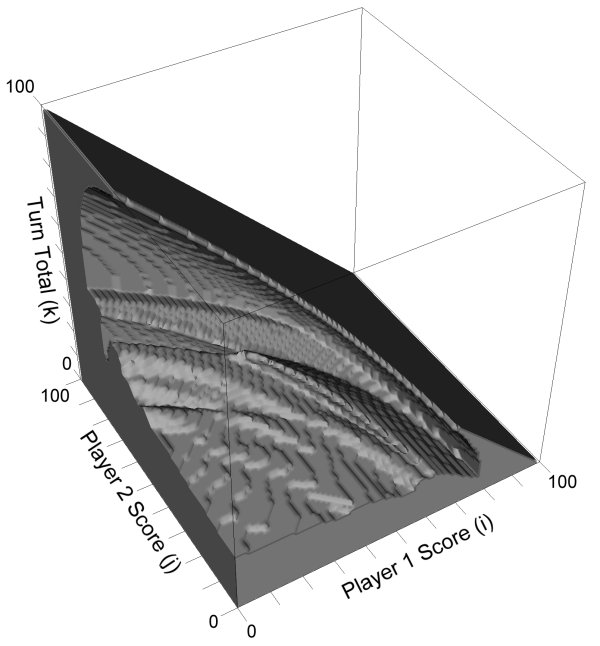
\includegraphics[width=0.5\textwidth]{neller_optimal_solution}
\caption{roll\slash hold boundary for the optimal Pig play policy (Neller)\label{figure1}}
\end{figure}
\begin{figure}
\centering
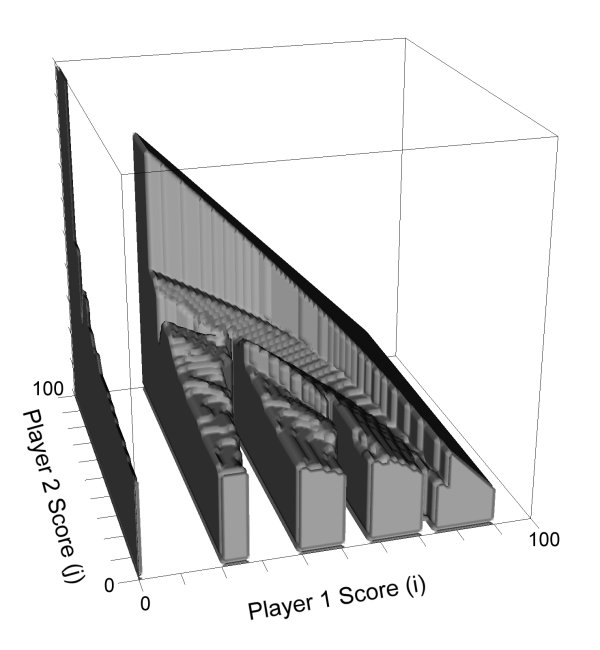
\includegraphics[width=0.5\textwidth]{neller_optimal_solution_2}
\caption{all of the states reachable by an optimal player (Neller)\label{figure2}}
\end{figure}


\subsection{Optimal Stratergy}
An optimal strategy is the strategy that when played against all other strategies is the best all-rounder.
It will beat most others more than half the time however may have a few weaknesses.
In the game of rock, paper, scissors, the optimum is to play each of the three choices about a third of the time.
However, in some game the optimum is to do something destructive. The optimum is not set out to get the best
win ratio but instead it wants to minimise the maximum loss an opponent can impose on it.
\\ \\In the world of pig there is a man called Todd W. Neller, who has 3 published papers on the matter.
One of them is all to do with the optimal strategy for the game of pig. As such the programme looks at all possible
game states within the pig dimension and at each node picks the one with the highest win likelihood.
We aimed to look at this in order to see whether we could get to Neller’s optimal with our own code,
or perhaps we get to a different optimal that may be better than Neller’s.
\\ \\The other possibilities for the optimal was to reach a pair of strategies that when played together existed in a Nash equilibrium.
A Nash equilibrium (named after Jordan Nash) is a point in a game space at which two strategies have to get worse against there opponent
in order to adapt from their current position. Because of this it would not be optimal to follow such a path and so they stay stuck in that state.
A good example of this is the prisoners game. It is defined as the following: \\
\textit{If you confess and your accomplice fails to confess, then you go free. If you fail to confess but your accomplice confesses, then you will be convicted and sentenced for the maximum term in jail. If you both confess, then you will both be convicted, but the maximum sentence will not be imposed. If neither confess, you will both be framed for another crime in which a conviction is certain.}\\

\begin{figure}
\centering
\includegraphics{prisoners_dilemma}
\caption{Prisoner's dilemma diagram\label{figure3}}
\end{figure}

As you can see the best outcome for each is that of no confession. However this is when one prisoner would look and say that confessing is the better
option for them and then does so. Because this scenario is played such that both prisoners cannot discuss it then they would both make this discussion
and you are left with the top left box after just a quick step. As you can see, this is not the best outcome for each of them, but they would have to
take a greater loss in order to reach the best outcome and so are stuck in this nash equilibrium.
\subsection{Preliminary Findings}
chris N

% Playing the game together

\section{Methodology}
\subsection{Group Organisation}
Mia
\subsubsection{Meetings}
\subsubsection{Creation of Project Plan}

\subsection{Coding}
\subsubsection{Similataneous Equations}

Anthony

% Outline how to solve for the probabilities by similitanious equations.

\subsubsection{Piglet}
When starting out on this project we were informed about a simpler version of pig, known as piglet. This is a version of pig
where by players take it in turns, flipping a coin until either a tail is flipped, or the player banks their turn score.
\\
\\
This simpler game contained all the same elements as pig but on a smaller scale. For starters it is a played with a coin rather than a die,
giving most probabilities as $\dfrac{1}{2}$ or multiples thereof, as opposed to the $\dfrac{1}{6}$ that you obtain via a die.
The other difference is that you typically only play to a score of $10$ compared to $100$ in pig.
These most simple of rule changes changed how the game works by a significant amount. % Disagree with this statement A LOT.
% The whole point is that it doesn't change how to game works so we can understand it and thus understand pig. Consider removing this sentence completely and check that what it is saying is not implied throughout the rest of the paragraph - Anthony
Since with a coin you may only score $1$ per flip meaning you must flip a minimum of $10$ times for you to reach you end goal. In pig this is not the case as you can roll anywhere from $2$ to $6$ points on a successful roll, giving you a minimum of $17$ rolls to achieve your goal. Having a change in the minimum number of flips allows luck to have a much greater presence in the outcome of the game, as we observed upon playing it ourselves. All of this made piglet the perfect first stepping stone to solving pig.

\subsubsection{Hand Written notes}
Since we had noticed pig was simpler we chose to use it as a way to achieve our first solution. We took pig and had it played to a total score of $3$. We played two strategies against each other; Strategy A was to bank on a turn score of $1$; Strategy B was to bank on a turn score of $2$; with both strategies banking as soon as they got over the winning score. From this we calculated all the simultaneous equations. This starts at the set that considers what the game state $P_{2,2,0}$ where by each strategy wins on its next go. These were solved using matrices like the one below.
%INSERT PICTURE OF MATRICES
From this we worked down through all possibilities to obtain the probabilities of each strategy winning from $P_{0,0,0}$ given they went first. This was the first theoretical answer we had achieved and had no idea of its validity.\\ \\
We repeated this process for a game to total score $2$ with both strategies being bank at $1$. We achieved another answer which looked relatively correct. As a group we noticed a pattern at this point to which the number of sets of simultaneous equations is that of the total score squared. It was here it was realised that working our piglet to $10$ would require $100$ sets of equations for which too much time would be wasted.

\subsubsection{Writing code}

% Required knowledge:
% - Similataneous equation sets
% - Matrix form of the sets

Once we had familisirised ourselves with the rules of the game, the equations, and
a few simple piglet examples, we moved to matlab.
The end goal is the make use of Matlab's computational power, to solve thousands of
similtaneous equations and find all the probabilites at each game state.
We can also make use of variable inputs to compare any strategy to another, and
even change the score needed to win and the dice probability.

Our first attempt at simply getting out ideas down as code was a very simplified
calculation of piglet. Although we coded in a dice probability variable that could be changed,
the code only worked for a dice flip, and when the variable was set to $\frac{1}{2}$.
It was also limited to taking in only Bank on strategies.
%Explain what Bank on strats are
We could however run to any winning score.

The way we got Matlab to solve the sets of similtanious equations was by turning them into
matrices of coefficients, variables and constants. $CX=D$ This was discussed before
and will be touched on again to talk about the layout of the matrices in the more general
refined code for pig.

By using the hand calculated simple piglet probabilities we could check to see if our
coded matrices were correct and fix any bugs. Once this was working we had our first
runnable code to get us going. We just had to generalise the code.
There were two steps to doing this; taking any strategy as an input, and having any
dice probability working in the code. The former was easier; an independent problem that we
made a function to do for us. The later was a little trickier but was a fundamental part
of building the matrices.

% Subsection on Strategies to matrices

% Subsection on coding matrices

...

Once we had done this, we had a generalised working code that could calculate the
probabilities of winning at any game state, for any two strategies, for any given
dice proability and to any winning score.

\subsubsection{Testing the code}

% Rhodri

To test the output of the code, we compared the calculated probabilities to experimental results. It was sufficient to test only the value in the lowest position in the matrix, $P_{0,0,0}$, since this value relies on the higher game-states (and therefore any errors in higher positions should be reflected in this output).

$P_{0,0,0}$ represents strategy A's probability of winning at the start of the game, assuming strategy A is the first to roll. To test this value, we simulated a series of games of pig with strategy A always being the first to roll, and outputted the number of wins for strategy A. For example, our $P_{0,0,0}$ for the input strategies ``bank on 20'' and ``bank on 21'' was 0.542626, indicating that ``bank on 20'' has a 54.26\% chance of beating ``bank on 21'' when going first. Running 1,000 series of 1,000 games gave us a distribution for the number of wins for ``bank on 20'' displayed in figure %ummm number?
. The median on the boxplot is very close to the projected probability which indicated that our code had correctly calculated $P_{0,0,0}$.

% Figure goes here please Liam :)

We similarly tested some more simple strategies with successful results. Then we tried to create awkward strategies that would test the limitations of our program. Of special interest were strategies that involved banking at turnscore 0, i.e. ``skipping'' a turn. In certain circumstances this decision could theoretically lead to a stalemate, where both strategies refuse to roll. While this would never happen in practical play, it was important to equip our Matlab script to deal with these scenarios so that it wouldn't cause issues when we later come to computer-generated strategies.

A particularly interesting example is a strategy which skips a turn whenever the two players' banked scores are equal. (For convenience we exclude the starting game-state where both players have score 0.) When this strategy plays against itself, around a quarter of games result in stalemates. But because the majority of games resulted in victories for one player, we still wanted to be able to analyse this strategy, and therefore had to update the code to accommodate stalemates.

The goal was that a stalemate would be counted as a loss for both players, since this is not a desirable outcome for our optimal strategy. Our modification therefore had the entire code run twice if a stalemate was detected. On the first run, every stalemate was declared a victory for player B (hence a loss for player A) to give an accurate recording of $P_{0,0,0}$. On the second run, we reverse the order of the strategies so that stalemates are counted as a victory for player A (hence a loss for player B), giving us an accurate value for $Q_{0,0,0}$.

Adjusting the script for simulating series of games to output the number of stalemates, we could then accurately test the $P_{0,0,0}$ and $Q_{0,0,0}$ values for strategies involving skips. Now satisfied that our code gave reliable outputs for any input strategies, we were ready to use this script to compare optimal strategies.

\subsection{Behavioural Economics}
Mia and Josh

\subsection{Statistical Testing}
\subsubsection{Fair test}
Throughout our project, we will be testing numerous different strategies against one and other to determine whether a strategy is better than another. To do this accurately, we will need to ensure that the test we conduct is fair and will give a reliable result.\\ \\
Say we were testing two strategies and played them against each other just once. Due to statistical inference, this test could give an unreliable result. Consider that you play the same strategy against itself for one game; there must be one winner, therefore the result will conclude that one strategy is better than the other, even though it’s the same strategy. Now say we were playing two different strategies where one was significantly better than the other, that doesn’t mean to say, that for all games played, the better strategy will always win. Again playing only one game of pig with these strategies may conclude that the worse game wins which would imply it is better than the other, even though we know this to be false. This is due to statistical inference.\\ \\
To reduce statistical inference, we will need to play numerous games of pig, say $n$ games. We will need to find an optimal value for $n$ to ensure that our result is as reliable as possible. By doing this we can find a reliable probability value for the strategies of winning against each other. We will calculate a confidence interval across a range of $n$-values on one strategy winning against itself. This would imply that the probability of the strategies winning are both 0.5. By running simulations in matlab, we can increase our value of n until the results are consistently within the confidence interval.
\subsubsection{Theory of Hypothosis testing}
Let $S$ denote a certain strategy within the game of pig.
Let $X$ denote the number of games won by that strategy after $n$ games.
As we will be playing $S$ against itself, we can say $E(X) =
\dfrac{n}{2}$, the expected amount of games $S$ should win against itself.
We can approximate $X$ to the binomial distribution to conduct the hypothesis test.
$X \sim Bin(n , p=0.5)$
By the binomial distribution

\begin{align}
E(X) &= np & SD(X) &= \sqrt{var(X)}\notag\\
&= \dfrac{n}{2} & &= \sqrt{np(1-p)}\notag\\
& & &= 0.5\sqrt{n} \notag
\end{align}
By using the $Z$ distribution at a 95\% confidence interval $(z=1.96)$, we compute the following interval.
\begin{align}
95\%Cl &= (\dfrac{n}{2} -1.96(0.5\sqrt{n}), \dfrac{n}{2} +1.96(0.5\sqrt{n}))\notag\\
&= (\dfrac{n}{2}-0.98\sqrt{n}, \dfrac{n}{2}+0.98\sqrt{n})
\notag
\end{align}
We would like the p value that we obtain to be within 95\% of the true value of the probability. For this system this implies that $0.475<p<0.525$. From the above interval for $X$, we can say that as $X=np$, using the upper and lower bounds for our $p$, we can then calculate a value for $n$, i.e. $0.475n$ would be equal to the lower bound of the confidence interval with $0.525n$ being the upper bound.
$$0.475n = \dfrac{n}{2} –0.98\sqrt{n}$$
Solving this for $n$, we get that $n=1537$. Similarly for the upper bound.\\ \\
This would imply that playing a game of pig $1537$ times would end up giving a probability of the strategies winning against each other that is within 95\% of the true value. As theoretical stats is not 100\% accurate, this theory was simulated in matlab. We tested this theory by running n games of pig $100$ times for a given strategy against itself, from n ranging from $1$ to $4000$, and calculating the $p$-value from each of the games.\\ \\
\begin{figure}
\centering
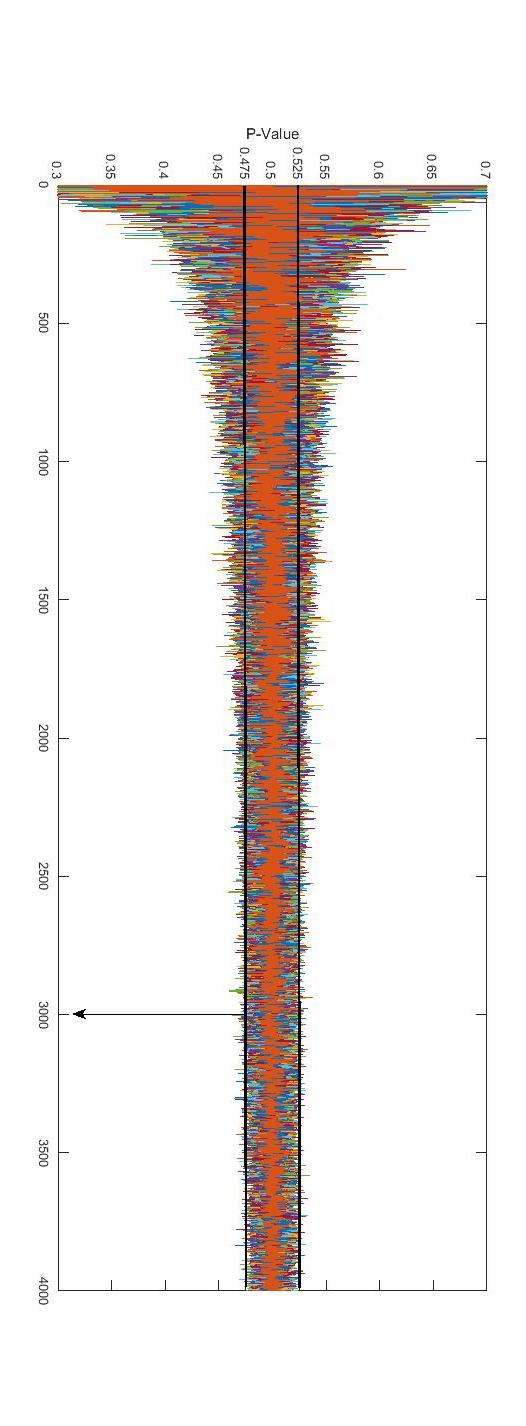
\includegraphics[height=24cm]{stats_testing}
\caption{stats testing\label{figure4}}
\end{figure}
Figure \ref{figure3} shows the distribution of the $p$-values over the number of games played. Each point on the $x$-axis has $100$ values for the $y$-axis. The orange colour that runs through the graph shows a higher concentration of values. This graph shows that the distribution for $p$ is scattered greatly for a small number of games played. We can see that around the $1500$ number of games played, the orange centre is located within the interval for $p$, marked by the two lines at $y=0.525$ and $y=0.475$, but there are still a lot of stray values. These stray values still occur, but less often, even when the number of games is large. By looking at the graph we can choose a value at which the majority of points lie within the interval. After the number of games passes $2500$, there doesn’t appear to be much decrease in the width of the distribution, so we will chose $3000$ as the appropriate number of games to play for a fair test.\\ \\
It would be a mistake to now only use $n=3000$ to test strategies. As the graph in figure \ref{figure3} shows, even for high values for $n$, you can still get stray results. Therefore, like what was done in the test to find $n$, for strategies we want to compare we will take $100$ results of $3000$ games. Then we can take the average of these results to further improve the reliability of the result.
\subsubsection{Running of tests}


\section{Findings}
\subsection{Pig}
\subsubsection{Did we solve Pig}
{\tiny YES.}

\subsection{Behavioural Economics}
\subsubsection{Do players stick to their risk preference}
\subsubsection{Players Interactions}

\subsection{Statistical Testing}
\subsubsection{Non-transitivity}
\subsubsection{Testing against our optimal}
\subsubsection{Testing against Nellers optimal}


\section{Conclusions}
\subsection{Overall findings}
\subsection{Determination of human affects on the optimal stratergy}
\subsection{Comparison to Nellers stratergy}

\nocite{*}
\bibliographystyle{alpha}
\bibliography{Pig_bib}
\end{document}
